%todo: {Accuracy of Registration} improve the perception of the MR view via accurate registration. Anatomy learning, personal information (gender, age, body shape)
\section{The User Specific Registration} \label{sec:3-PPMM:Registration}
The main advantage of the magic mirror framework is to create a personal AR visual effect, which build a link between the user's own body and the medical information. Registration is the most important part to forge an AR view of the user's body and a satisfactory non-physical visual effect.
It includes to select the corresponding medical information from the database and transform the selected data to fit the user's body to create valid magic mirror effect (see \figurename{\ref{fig:3-MMC:MedicalInfoFlow}}). Via the color and depth camera, the system can detect the personal information (e.g., gender, age, height and so on) to select the best medical information for current user and transform it as needed. However, the detection of personal information is mainly based on machine learning and just calculate a general acceptable result. For some important issue, the interactive registration is introduced to improve the accuracy of the magic mirror AR view.
A personal perception of the medical information is the major object of magic mirror, and it includes two parts: (i) correct medical information for current user and (ii) accurate registration of the non-physical visual effect. In this section, personal information detection and interactive registration are discussed to create a personal perception of anatomy for medical learning.

\subsection{Personal Information Detection}
After a long time use of the Magic Mirror system in the real scenario, we could figure out that the Magic Mirror system is still imperfect. As the different between children and adults, male and female, young and elders, the non-physical visual effect should have some difference. Therefore, lack of the personal information makes the using of the system limited. One of the problem is that sometimes it has to be used under the supervision since some parameter of the user need to be input manually. 
If it has more accurate personal information of the user, a better medical data would be applied on the user's body and generates a more satisfactory AR view.
To allow an accurate and rational augmentation of the medical data, the gender, age, body size and pose of the user can be detected using the biometric recognition, skeleton tracking, and 3D reconstruction libraries. Then the corresponding medical volume is selected, transformed, and augmented onto the user body. 

\subsubsection{Personal Information to collect}
The Kinect is the only sensor to observe the user and all the parameter of the user is detected via the color/depth image and the skeleton (see \figurename{\ref{fig:3-PRMM:BiomatricInformation}}). If a new user is detected in the valid range of the system, the system goes to the stage of parameters detection and calculate all the parameters. The following list are the parameters we plan to detect from every user, including gender, age, height, length of the limbs, 3D volume, weight, circumference, and body shape.
\begin{enumerate} [label=\arabic*.]
	\item  Gender and age: Figure out the male or female of the user, detect the child, young, adult and elder people.
	\item  Height and length of limbs: Compute the high and limbs length of the user in millimeter.
	\item 3D volume: Reconstruct the 3D volume of the user. The volume is the upper part of the user's body as it is enough for the information extraction and the volume information of the legs and feet are not needed.
	\item  Weight: Approximate estimate the weight of the user.
	\item  Circumference: After obtain the upper part of the 3D volume, measure the circumference of the bust, waist and hip information of users.
	\item  Shape: Give the shape information of users by the WHR (waist-hip ratio) index.
\end{enumerate}
\begin{figure}
\centering
\includegraphics[width=0.7\linewidth]{figures/3-PRMM/BiomatricInformation}
\caption[Biomatric Information]{Biomatric Information tree}
\label{fig:3-PRMM:BiomatricInformation}
\end{figure}

\subsubsection{system design}
In this section, we want to improve the recognition of users for an Augmented Reality Magic Mirror system by the simple computer vision and machine learning methods. The purpose of the present thesis project is implementing a middle-ware software to provide the user's personal information to the Magic Mirror system by the automatic recognition. Gender, age, height, length, weight, volume, circumference and body shape of the user are detected by the middleware, and then application based on this framework can extent the system with smarter and more interesting features. 

The idea of personalizing the Magic Mirror system is to develop a middleware, which works as the user recognition layer to collect the personal user infromation  based on the color image, depth and skeleton stream from the Kinect sensor. Through the whole processing of the user recognition, the middleware provides all the information of the user as parameters to the Magic Mirror framework. All these parameters would help the system generate a better result of the Augmented Reality. The middleware between the layer of hardware and the application of the Magic Mirror is an independent and automatic recognition software. All the parameters provided for the Magic Mirror system by the user recognition middleware would be discussed in the section.
\begin{figure}
	\centering
	\includegraphics[width=0.7\linewidth]{figures/3-PRMM/middlewareFramework.png}
	\caption{Recreate this figure based on the final magic mirror framework.}
	\label{fig:3-PRMM:middlewareFramework}
\end{figure}

An independent middleware is designed to collect personal user information while not affect the basic interaction of the Magic Mirror system. The middleware does not involve the non-physical visual effect definition and basic interactions between the user and Magic Mirror system. The procedure of the automatic recognition would take several minutes as the user need to be scanned by the sensor totally.  Once the middleware detects a user within the valid range of the system, it starts to recognize the information of the user and the whole procedure of the iteration is described as \figurename{\ref{fig:3-PRMM:InteractionWithMiddleware}}.
The first step of using the middleware software is as same as the Magic Mirror system. The first task is user detection, to check if there is a new user in the view of the system. The user of the system is just standing in front of the display. But in this time, the system would not give any output of Augmented Reality result on the monitor. When the user stands upright, the system detects the gender, age, height and limbs length immediately without any movement of the user. 

After that, the second step is different. In this step, the user of the system need to turn a circle in front of the sensor in order to make the sensor of the system scan the user's body totally. When the user is turning around, the monitor of system would tell the user moves slowly and continuously. When the user finish the movement, the system would complete the collection of the personal user information. If the user don't satisfy the result of the reconstruction, the system make a hint to repeat the whole procedure.
\begin{figure}
	\centering
	\includegraphics[width=0.7\linewidth]{figures/3-PRMM/InteractionWithMiddleware.png}
	\caption{Workflow of the interaction with the middleware to collect the personal information}
	\label{fig:3-PRMM:InteractionWithMiddleware}
\end{figure}

In order to achieve the goal of automatic user's information detection, an Open Source Biometric Recognition framework is chosen to detect the gender and age from the captured color images. At meanwhile, the OpenNI and NITE libraries are adopted in this system for the height and limb length calculation. Besides the above parameters, Weight, volume, circumference and body shape are all based on the 3D reconstruction of the user's upper body, which is done by the 3D reconstruction SDK and OpenCV\footnote{\url{http://opencv.org/}} libraries. 
After the detection of the user, all the information talked above would be prepared as the parameters for the Magic Mirror system. Combining all of these functions, the personal user information would be collected efficiently and stably. 

%like gender, age, height, length of limbs and 3D volume. The weight of the user comes from the volume calculation of the 3D module. The circumference is a cut calculation of the 3D volume information along the Z axis. The size or shape infor-mation of the user extended by the ratio between the circumference information of waist and hip. The whole interaction of each function in the middleware system are clear at here.

\subsubsection{Implementation}
The Open Source Bio-metric Recognition (OpenBR)\footnote{\url{http://openbiometrics.org}} is employed to realize the functions in the biometrics recognition \cite{Klontz2013}. The basic algorithm used in the OpenBR is the Spectrally Sampled Structural Subspaces Features (4SF) algorithm. The algorithm is based on the statistical learning methods and used in the field of demographics and aging of the face recognition at before.
In this section, the system is designed to use the 3D reconstruction technologies to reconstruct a 3D model of the user's upper body and then obtain more personal details with the 3D reconstruction model for the purpose of further analyses. ReconstructMe SDK \footnote{\url{http://reconstructme.net/reconstructme-sdk/}} is a powerful and affordable real-time 3D reconstruction system.
Combining all the following functions, the personal user information would be collected efficiently and stably. The Magic Mirror system could refer to the user's information as personalized parameters and gives us more useful and interesting applications.
\begin{figure}
	\centering
	\includegraphics[width=0.7\linewidth]{figures/3-PRMM/OpenBR.png}
	\caption[OpenBR]{Overview of openBR Capabilities}
	\label{fig:3-PRMM:OpenBR}
\end{figure}
%In the computer vision and computer graphics, 3D reconstruction is a classical problem and being one of the fundamental problem within many applications. After many years later, this problem still gains considerable attention and as an active research area in the computer vision field. Even now, reconstruction of the geometry structures and the texture of the object from a sequence and aligned images is still a challenge. The real-time processing time and high revolution of qualities are still under research. 

\paragraph{gender and age}
We adopt the OpenBR framework to help us in the face detection and recognition. The algorithm of face detection used in the OpenBR framework needs to detect the eye position and find the face within the image. To get more accurate result, the system should capture a clear front face image of the user. 
%From the publication, we know that this framework incorporates more methods published in the last five years and it is always maintained by the background group. It is easy to use and the experiment result shows us that in the gender and age classification part, there are 92.8\% accuracy of the gender estimation, 9.9 years RMS error of males and 12.8 years RMS error of female.
All the works like detection, normalization, representation and extraction are done by the OpenBR framework. What the middleware does is to implement a thread using the framework. When the user stands in front of the system, the system firstly estimates the rotation of the human body. When the user faces the camera, the image is captured automatically. After the capturing, the image including the front face goes to the engine of the OpenBR framework, and then the gender and age are calculated.
\paragraph{Height and length of limbs}
From the basic understanding of the word human height, we all know that the height is the distance from the top of the head to the bottom of the feet. As we already have the user's information and the depth image, the coordinate of the top point of the user is very easy to get. 
As the feet sometimes may not be seen by the Kinect sensor, the height would be converted to the distance from the top of the head to the ground.
Thanks to the help of the OpenNI and NITE SDK platform, the plane function of the floor could be easily assessed from the depth image and the user map is generated, defining the valid pixel belonging to the user's body in the depth image.
For the length of limbs, there are four values need to be calculated, LeftArmLength, rightArmLength, leftLegLength and rightLegLength. The user could be asked to keep a cross pose to get a clear view of the body and limbs. The limb length is the sum of the distances between corresponding skeleton joints.

\paragraph{3D volume}
The ReconstructMe framework is used to implement the 3D volume reconstruction and the work-flow of the reconstruction is shown in \figurename{\ref{fig:3-PRMM:bodyReconstruction}}. One important task of the body reconstruction is to estimate the rotation angle of the user's body. If the total rotation angle of the user is less than $360\degree$, it means that the user hasn't been constructed and the system goes to reconstruct. The system tries to get the new position of the user, transforms the previous position to the new one and copies the data. After the transformation, it gets the next depth frame and repeat the reconstruction frame by frame until the sum of the angle larger than 360 degree, which indicates that the user has totally scanned. However, the procedure of the reconstruction would end if the tracking failed.
\begin{figure}
\centering
\includegraphics[width=0.7\linewidth]{figures/3-PRMM/bodyReconstruction}
\caption{Flowchart of the reconstruction procedure}
\label{fig:3-PRMM:bodyReconstruction}
\end{figure}

\paragraph{Weight}
Weight is an important characteristic of human beings as the height. Machine learning could be one of the solutions is to estimate the weight of a human body. The height, length of limbs, bust size, waist size, hip size and other biometric information cloud be considered as the input features for the weight learning. Lack of a valid huge database makes us give up this method. 
In the proposed middleware, we provide the simple method to estimate the weight information of the user. It is a simple idea that the weight comes from the volume of the 3D reconstruction. After the 3D reconstruction, a watertight 3D mesh is created and the volume is calculated.

Duo to the limitation of the Kinect sensor in the field of views, the 3D volume reconstructed cannot cover the whole body. However, we could just use the upper body of the user to estimate the full weight. As the result presented by \cite{Tozeren2000}, the upper body is about 68.2\% of the full in the human's weight. It becomes very easy to get the hull weight, if we have the weight of the upper. No matter how the reconstructed result is, the upper body is composed of the result of the 3D reconstruction which without the part below the hip. As the hip joint information is known, we just make a cut from the hip position and generate a new volume without the hips.
As the density of human body is very near to the density of water ($1.0 g/cm^3$), the weight of user in the system would be as same as the volume.
\begin{equation}
Weight = (Volume * Density)/0.682
\end{equation}

\paragraph{Circumference and Body Shape}
After the obtainment of the 3D body volume of the user, the last measurement is to get the information of the user's shape like the circumference of bust, waist and hip. The 3D volume is just a reconstructed model of the object and the further implementation is based on it.
From the reconstructed 3D volume, the body surface can be calculated easily. The circumference of the circle in each layer gives us the information of the user's body shape. As shown in \figurename{\ref{fig:3-PRMM:Circumference}}, it is a simple example of the user's body when we look at the volume in the middle layer from the cross-sectional view. The blue circle is the Z axis cut on 3D volume and the length of the cut would refer to the circumference on that layer.
\begin{figure}
	\centering
	\includegraphics[width=0.5\linewidth]{figures/3-PRMM/Circumference}
	\caption{The circumference of the circle in each layer in the 3D body volume gives us the information of the user's body shape.}
	\label{fig:3-PRMM:Circumference}
\end{figure}
The key point at here for the body shape detection is how to find the right layer for the right circle we want. The bust, waist and hip are the most important parameters for the body shape detection within the whole Magic Mirror system. Because the volume of the 3D model is constructed by layer one by one, if we know the right position of the bust, waist and hip, we could refer to the correspondent layer of them and acquire the length of each parameters.
For the length detection, we have already used the joints information. Right now, for the bust, waist and hip detection, the neck joint, torso joint and hip joint are under consideration.
The circumference in the shoulder joint is the shoulder circumference. As the same idea, the bust is in the middle between the shoulder and torso. The waist is in the middle between the torso and hip. The hip is the layer refer the position of the hip joint as well.

Body shape information of the user refers to the index of health and the risk of developing serious health conditions. We introduce the Waist-Hip-Ratio (WHR)\cite{Consultation2008} to indicate the condition of obesity for the system's users. we could know that the “apple shaped” bodies would be more healthy than the “pear shaped” as the “apple shaped” bodies has less weight around the waist makes the value of WHR smaller than the “pear shaped” bodies.
The system would provide the value of Waist-Hip-Ratio index to the user and indicate the health condition of them.

\subsection{Interactive Registration}
The skeleton output from Kinect limits the precision of the AR magic mirror applications. Thus, our magic mirror augmentations would contain errors and users would easily distinguish anatomical offsets on their body resulting in a poor anatomy learning environment. Alternatively, we had considered projectors to display human anatomy and along with their existing limitations the same inaccuracies would exist \cite{Sun2013}. Interactive solution can be proposed to improve the registration as the magic mirror system always takes the user movement as input.
Our aim was then to propose a method to correct for such overlay inaccuracies that could be translated to any magic mirror system worldwide. 

\subsubsection{Anatomical bone landmarkers}
Together with orthopedic surgeons, we have defined five bone landmarks that (i) users can easily identify and touch while standing in front of the Kinect, and (ii) that are accurately and easily identified in medical data such as CT \cite{ma2013ismar}. These are: left and right acromion, left and right anterior superior iliac spine, and the manubrium (see \figurename{\ref{fig:3-PRMM:bonelandmarker}}).
\begin{figure}[htb]
	\centering
	\label{fig:3-PRMM:bonelandmarker}
	\includegraphics[width = 0.75\linewidth]{figures/3-PRMM/FiveBoneLandmarker.png}
	\caption{Selected anatomical points for Kinect skeleton improvement and subsequent CT warping and interpolation.}
\end{figure}

Prior to correctly using our AR magic mirror system, the users stand in front of the monitor and we displayed virtual marks near the five bone landmarks. The users are asked to interactively adjust the positions of the five marks to fit their own bone positions. In addition, the exact locations in the VKH CT dataset of the five selected bone landmarks are known. A linear interpolation was executed to estimate the torso point (i.e. a $6^{th}$ landmark) in the CT volume to improve the overlay. Then the scale factors and transformation matrix were computed to render the anatomical image onto the user's body. These landmark positions allow the deformation and interpolation of the medical data correctly within the magic mirror and onto the human body, resulting in a more precise augmentation. A user study involving surgeons and anatomy experts confirmed our findings and will be presented in the following section.
%%%%%%%%%%%%%

%tranditional way to do the registration
\subsubsection{Improvement of Kinect skeleton}
We presents a general method to interactively improve and correct the Kinect skeleton for anatomy education purposes. We believe that our general method can be applied to projectors or other sensors as well for augmented reality. A thorough validation of our method demonstrated improved precision of anatomical landmarks and opens the avenue to future improvements in medical education. 
\figurename{\ref{fig:3-PRMM:5Joints}} shows a comparison between the traditional Kinect skeleton and its proposed improvement. The first row depicts visually the exactness of the new skeleton. The second row depicts the skeleton landmarks directly on CT data. We observe that the shoulder and anterior superior spine are inaccurate in the images. The last row depicts the selected bone landmark positions within CT as well. Transverse and sagittal CT slices of the visible human Korean are seen respectively in rows 2 and 3.

To improve the perception of the AR view, the medical data has to be registered to the current user. A simple method used by the magic mirror framework is that an anatomy doctor helps to find the corresponding Kinect skeleton joints in the CT volume (see \figurename{\ref{fig:3-PRMM:5Joints:a}} and \figurename{\ref{fig:3-PRMM:5Joints:c}}). The point 1-5 are raw Kinect skeleton joints and slice 1-5 are estimated by doctor according to the yellow line draw on user's body using the raw Kinect skeleton joints information. So the scaling factor from CT volume to the current user is:
\begin{equation}
	WidthScale = Avg(\frac{{{W_{12}}}}{{W_{12}^{CT}}},\frac{{{W_{34}}}}{{W_{34}^{CT}}})
\end{equation}
\begin{equation}
	HeightScale = Avg(\frac{{{H_{14}}}}{{H_{14}^{CT}}},\frac{{{H_{23}}}}{{H_{23}^{CT}}})
\end{equation}
$T_{K\_CT}$ is the transformation from Kinect coordinate system to CT volume. $T_{K\_n}$ and $T_{CT\_n}$ is the transformation matrix from original point in Kinect world and CT volume to the skeleton joint $n$, correspondingly.
\begin{equation}
	T_{K\_CT} = T_{K\_5} * T_{CT\_5}.inv()
\end{equation}
\begin{figure} 
	\centering
	\subfloat[~Kinect skeleton]{ \label{fig:3-PRMM:5Joints:a}
		\includegraphics[height = 6cm]{figures/3-PRMM/Kinect5Joints.png}
	}
	\subfloat[~Improvement of Kinect skeleton]{ \label{fig:3-PRMM:5Joints:b}
		\includegraphics[height = 6cm]{figures/3-PRMM/Kinect6Joints.png}
	}
	\quad
	\subfloat[~Skeleton joints in CT volume]{ \label{fig:3-PRMM:5Joints:c}
		\includegraphics[width = \linewidth]{figures/3-PRMM/Kinect5JointsCT.png}
	}
	\quad
	\subfloat[~Bone landmarker in CT volume]{ \label{fig:3-PRMM:5Joints:d}
		\includegraphics[width = \linewidth]{figures/3-PRMM/Kinect6JointsCT.png}
	}
	\label{fig:3-PRMM:5Joints}
	\caption{The inaccurate Kinect skeleton (a) The point 1-5 are raw Kinect skeleton joints. (b) The inaccurate Kinect skeleton, in yellow, compared to the improved Kinect skeleton positions in red. The points 1'-5' are the position of the five selected bones, which are suggested by doctor.(c) Slice 1-5 are estimate by doctor according to the yellow line draw on user's body using the Kinect skeleton joints information. (d) Slice 1'-5' are the selected five bone suggested by doctor and the slice 6', which are computed from slice1'-5', is corresponding slice for joint 6'.}
\end{figure} 

The goal of the proposed method is to create a more precise user-specific AR overlay environment. The positions of the anatomical bone landmarks can improve the deformation and interpolation of the medical data, resulting in a more precise Kinect skeleton and augmentation. A user study involving surgeons and anatomy experts confirm our findings. The following scale factors were calculated for the improved system via the selection bone landmarks.
\begin{equation}
WidthScale = Avg(\frac{{{W_{1'3'}}}}{{W_{1'3'}^{CT}}},\frac{{{W_{4'5'}}}}{{W_{4'5'}^{CT}}})
\end{equation}
\begin{equation}
HeightScale = Avg(\frac{{{H_{1'5'}}}}{{H_{1'5'}^{CT}}},\frac{{{H_{3'4'}}}}{{H_{3'4'}^{CT}}},\frac{{{H_{2'4'}}}}{{H_{2'4'}^{CT}}})
\end{equation}
$T_{K\_n'}$ and $T_{CT\_n'}$ is the transformation matrix from original point in Kinect world and CT volume to the bone marker $n'$, correspondingly. Using Eq.\ref{eq:3-PMRR:6CT}, the position of the torso in the CT volume is calculated.  
\begin{equation} \label{eq:3-PMRR:6CT}
T_{CT\_6'} = Avg(T_{CT\_n'} * T_{K\_n'}.inv() * T_{K\_5 })
\end{equation}
\begin{equation}
T_{K\_CT'} = T_{K\_6'} * T_{CT\_6'}.inv()
\end{equation}

\subsubsection{Evaluation}
As an augmented reality anatomy learning application, both accuracy and system usability are very important prior to its translation in classroom. We undertook one user study with particular users having expert anatomy knowledge to evaluate if this system is precise enough for anatomy learning and the proposed method improve th accuracy of the AR view.
\paragraph{Assessing the magic mirror system precision and usability}
\textbf{Participants}: Seven participants were included in this study (two surgeons and five final year undergraduate medical students). 
Analysis: a Likert scale was used which is a type of psychometric response scale often used in surveys and the most widely used scale in survey research. When responding to a Likert questionnaire item, respondents specify their level of agreement to a statement. The format of our 5-pt Likert was: (1) \textit{strongly disagree}, (2) \textit{disagree}, (3) \textit{neither agree nor disagree}, (4) \textit{agree}, (5) \textit{strongly agree}. 

To assess the precision of our personalized magic mirror we asked the participants to interact with the system platform which integrates user-specific anatomical landmark selection. Participants were asked to provide an estimated numerical offset, if any, on how far specific bone landmarks or organs were with respect to their own body. For this, they interacted with the magic mirror window, CT data, and used their own medical knowledge and expertise for judgment. CT data was displayed in an interface depicting both transverse and sagittal planes, and participants would quantify the offsets. If needed, a ruler was provided to assist them. The anatomical targets during evaluation were defined as: the anterior superior iliac spine, manubrium, heart, and liver. Results from this exercise are shown in \tablename{\ref{tb:3-PRMM:results1}}, with offsets measured in centimeters. Results from the user study show that the precision of user-specific learning environment is on average 0.96cm.
\begin{table}
	\caption{Precision (in cm) of magic mirror system based on anatomical offsets}
	\label{tb:3-PRMM:results1}
	\scriptsize
	\begin{center}
		\begin{tabular}{p{4cm}|p{3cm}|p{4cm}}
			Anatomy & Offset (Mean$\pm$STDev) & Improved Offset (Mean$\pm$STDev) \\
			\hline
			anterior superior iliac spine & $6.83\pm4.97$ & $0.67\pm0.52$\\
			manubrium & $3.17\pm1.72$ & $0.67\pm0.75$ \\
			heart & $1.83\pm1.47$ & $1.17\pm1.60$\\
			liver & $5.08\pm2.42$ & $1.33\pm1.21$
		\end{tabular}
	\end{center}
\end{table}

The seven participants were then asked to judge the usability of the AR magic mirror system by responding to the following questions: (i) is the overlay accurate w.r.t human body (ii) is the user interface easy to use, (iii) is it fun to play, (iv) can it be used for medical education, and (v) would it have stronger impact for medical education learning?
The Likert scale results for the first four questions are shown in \tablename{tb:3-PRMM:results2}.
\begin{table}
	\caption{Likert scale results regarding magic mirror usability}
	\label{tb:3-PRMM:results2}
	\scriptsize
	\begin{center}
		\begin{tabular}{p{6cm}|p{3cm}}
			\space & Mean$\pm$ STDev \\
			\hline
			is the augmented reality overlay accurate w.r.t human body & $4.00\pm0.89$\\
			is the user interface easy to use & $3.67\pm1.03$ \\
			is it fun to play & $4.50\pm0.55$\\
			can it be used for medical education & $4.17\pm0.75$
		\end{tabular}
	\end{center}
\end{table}

For the last question regarding the impact of our technology, there was a unanimous response that the AR magic mirror system should be considered as a potential platform to complement existing anatomy learning tools inside anatomy classrooms. 
\subsubsection{Discussion}
The precision of our method is visually demonstrated in \figurename{\ref{fig:3-PRMM:ResComparing}}. We observe that the acromion and anterior superior iliac spine, using the traditional Kinect skeleton, is not positioned correctly within the CT data compared to the modified Kinect skeleton version (1-2 vs. 1'-2'; 3-4 vs. 3'-4'). The orthopedic surgeons participating in our study confirmed this.
\begin{figure}[htb]
	\centering
	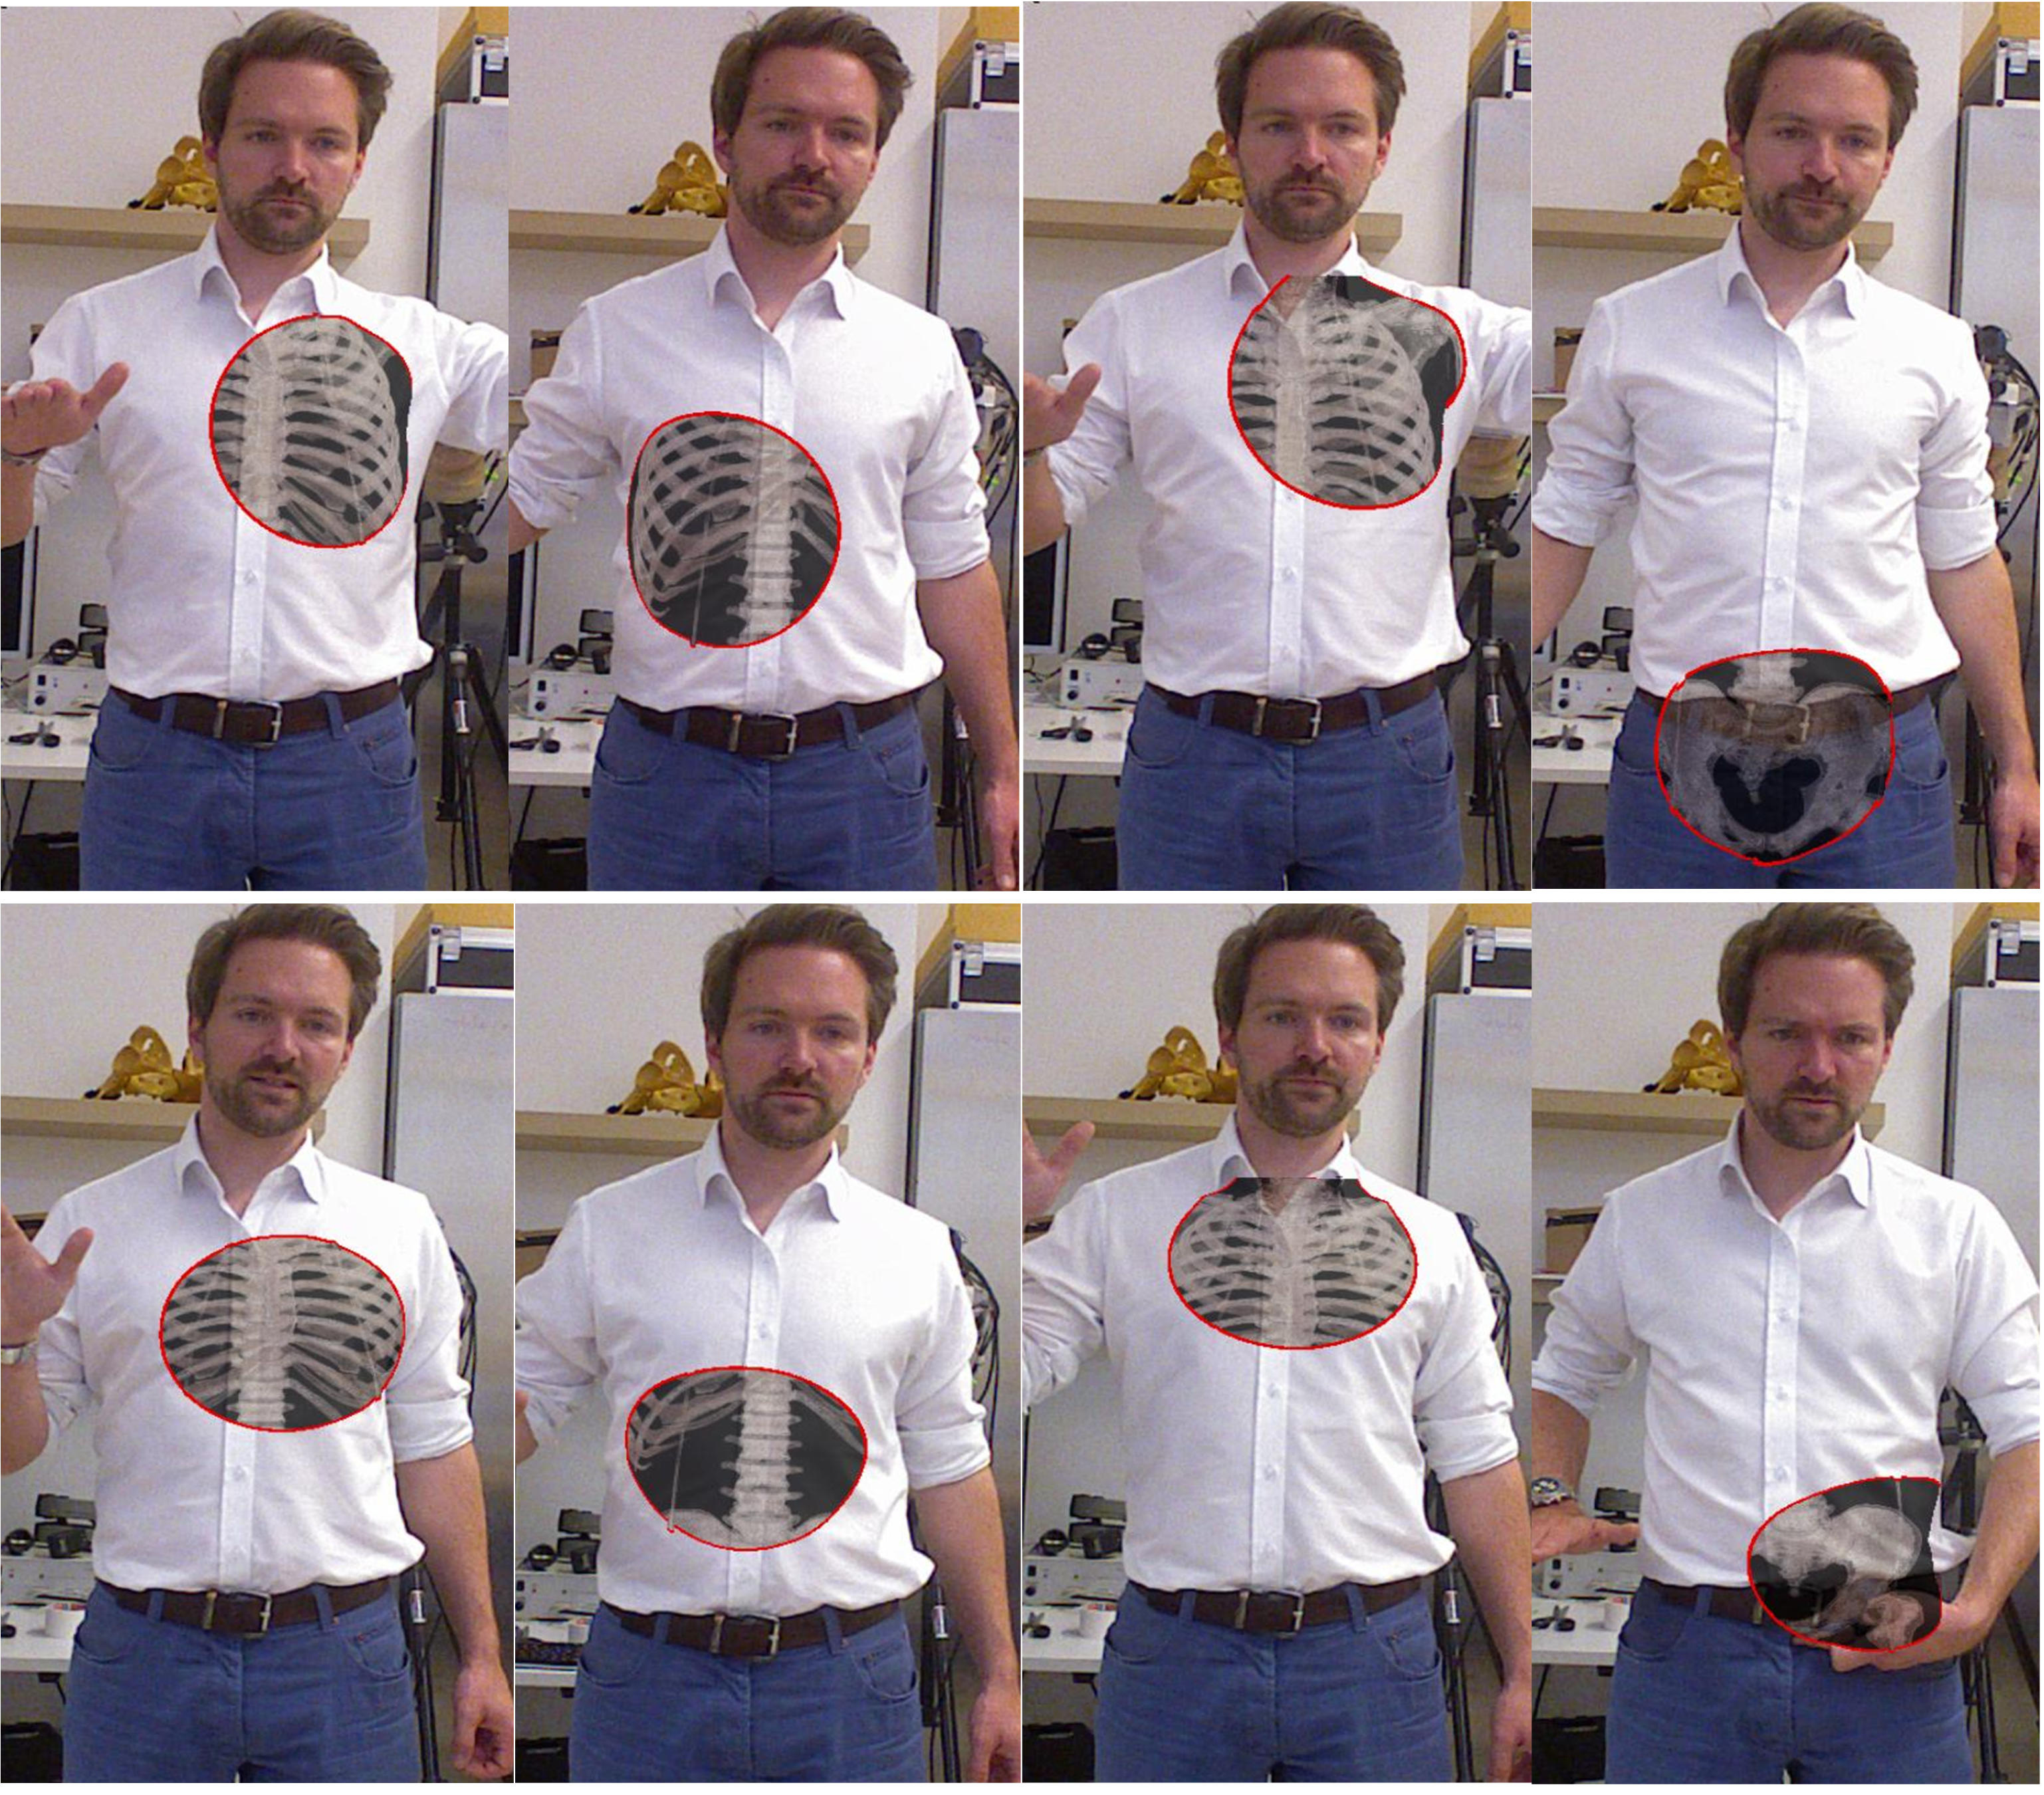
\includegraphics[width = \linewidth]{figures/3-PRMM/ResComparing.png}
	\label{fig:3-PRMM:ResComparing}
	\caption{Figure 4:	The magic mirror before (top) and after (bottom) the Kinect skeleton adjustment. Column 2 depicts the bottom of the rib cage being positioned correctly after skeleton correction.}
\end{figure}
Results from a user study show the impact of interactively improving the Kinect skeleton to increase precision for a better visualization of anatomy. The offsets of specific anatomical landmarks decreased significantly. The following comments were collected:
\begin{enumerate}
	\item the precision improved; making the user touch anatomical landmarks is cool since this is the way it is done in clinic…
	\item two additional landmarks easily accessible are the sternum and bottom of rib cage…
	\item make the magic mirror circle bigger for larger anatomy…
	\item voice command is a good idea but it is sensitive to the surroundings voice
	\item interactions between observers …
	\item could introduce the female CT visible human Korean…
	\item could use a healthy patient CT or other modality…
	\item could make the CT slices bigger on the screen…
\end{enumerate}